%Optics Homework_6
\documentclass[10pt,a4paper]{article}
\usepackage[UTF8]{ctex}
\usepackage{bm}
\usepackage{amsmath}
\usepackage{amssymb}
\usepackage{graphicx}
\title{光学作业\#6}
\author{陈稼霖 \and 45875852}
\date{2018.12.18}
\begin{document}
\maketitle
\section*{4-5}解:
自由传播时轴上场点的振幅为$A=\frac{1}{2}A_1$,光强为$I=A^2=\frac{1}{4}A_1^2$,其中$A_1$是第一个半波带在轴上场点产生的振幅,将各半波带在轴上场点产生的振幅近似等于第一个半波带周围的半波带在轴上场点产生的振幅。

\textbf{a}屏在轴上场点产生的复振幅如振动矢量图\ref{OpticsHomework_6_4-5a}所示
\begin{figure}[h]
\centering
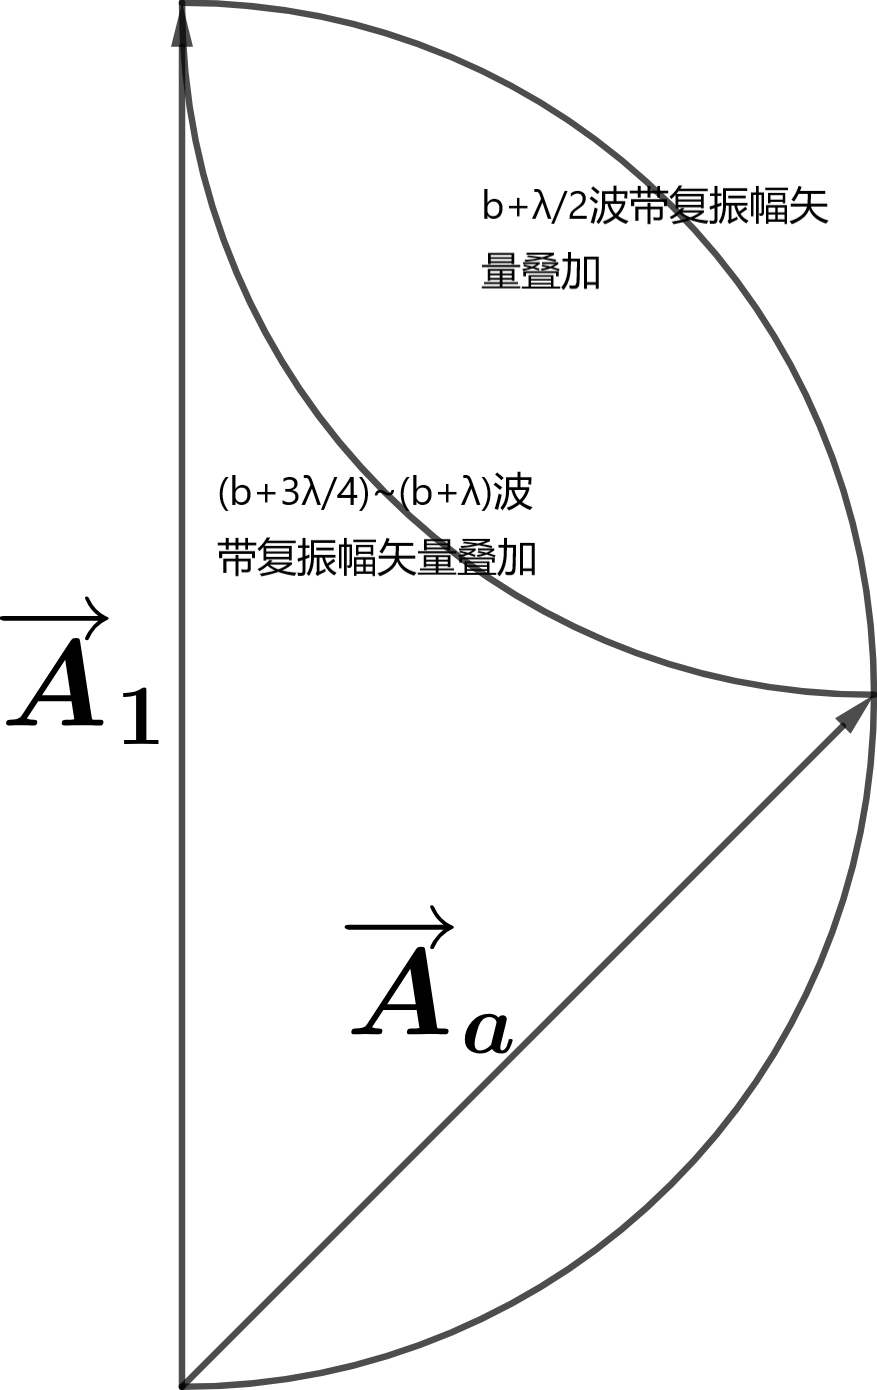
\includegraphics[scale=.12]{OpticsHomework_6_4-5a(tailored&marked).png}
\caption{4-5a}\label{OpticsHomework_6_4-5a}
\end{figure}

\noindent 得到轴上场点的振幅为$A_a=\frac{\sqrt{2}}{2}A_1$,光强为$I_a=A_a^2=\frac{1}{2}A_1^2$,与自由传播时之比为$\frac{I_a}{I}=2$。

\textbf{b}屏在轴上场点产生的复振幅如振动矢量图\ref{OpticsHomework_6_4-5b}所示
\begin{figure}[h]
\centering
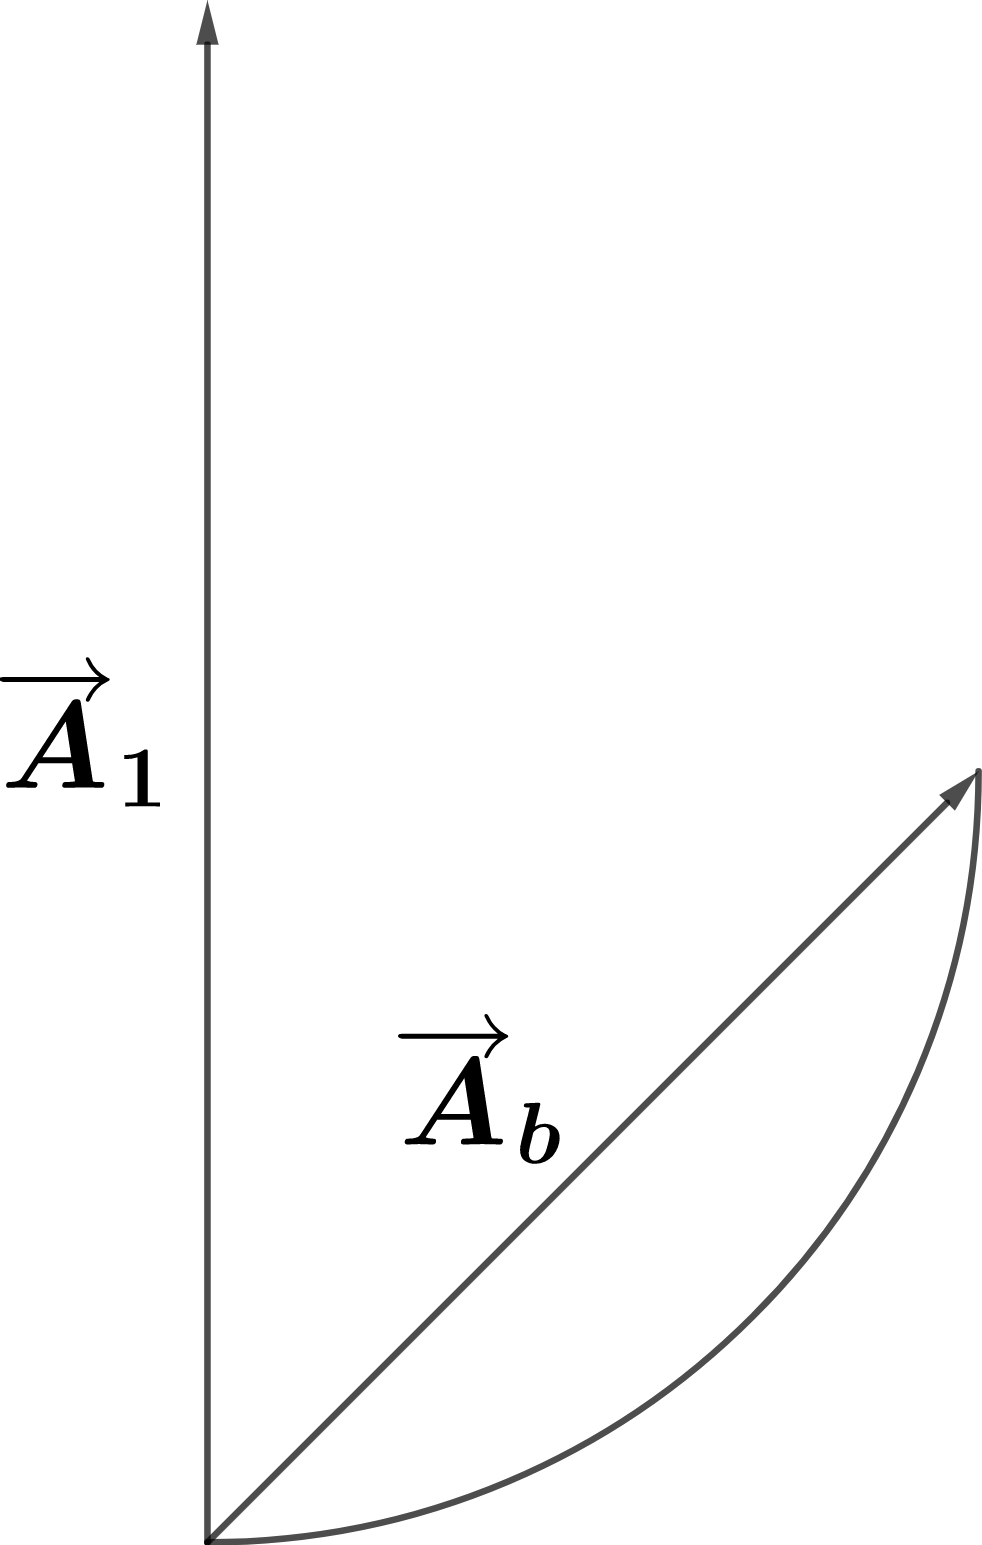
\includegraphics[scale=.1]{OpticsHomework_6_4-5b(tailored).png}
\caption{4-5b}\label{OpticsHomework_6_4-5b}
\end{figure}

\noindent 得到轴上场点的振幅为$A_b=\frac{\sqrt{2}}{2}A_1$,光强为$I_b=A_b^2=\frac{1}{2}A_1^2$,与自由传播时之比为$\frac{I_b}{I}=2$。

\textbf{c}屏次波源面积较自由传播减半,则在轴上场点的振幅也减半,$A_c=\frac{1}{2}A=\frac{1}{4}A_1$,光强为$I_c=A_c^2=\frac{1}{16}A_1^2$,与自由传播时之比为$\frac{I_c}{I}=\frac{1}{4}$。

\textbf{d}屏在轴上场点产生的复振幅如振动矢量图\ref{OpticsHomework_6_4-5d}所示
\begin{figure}[h]
\centering
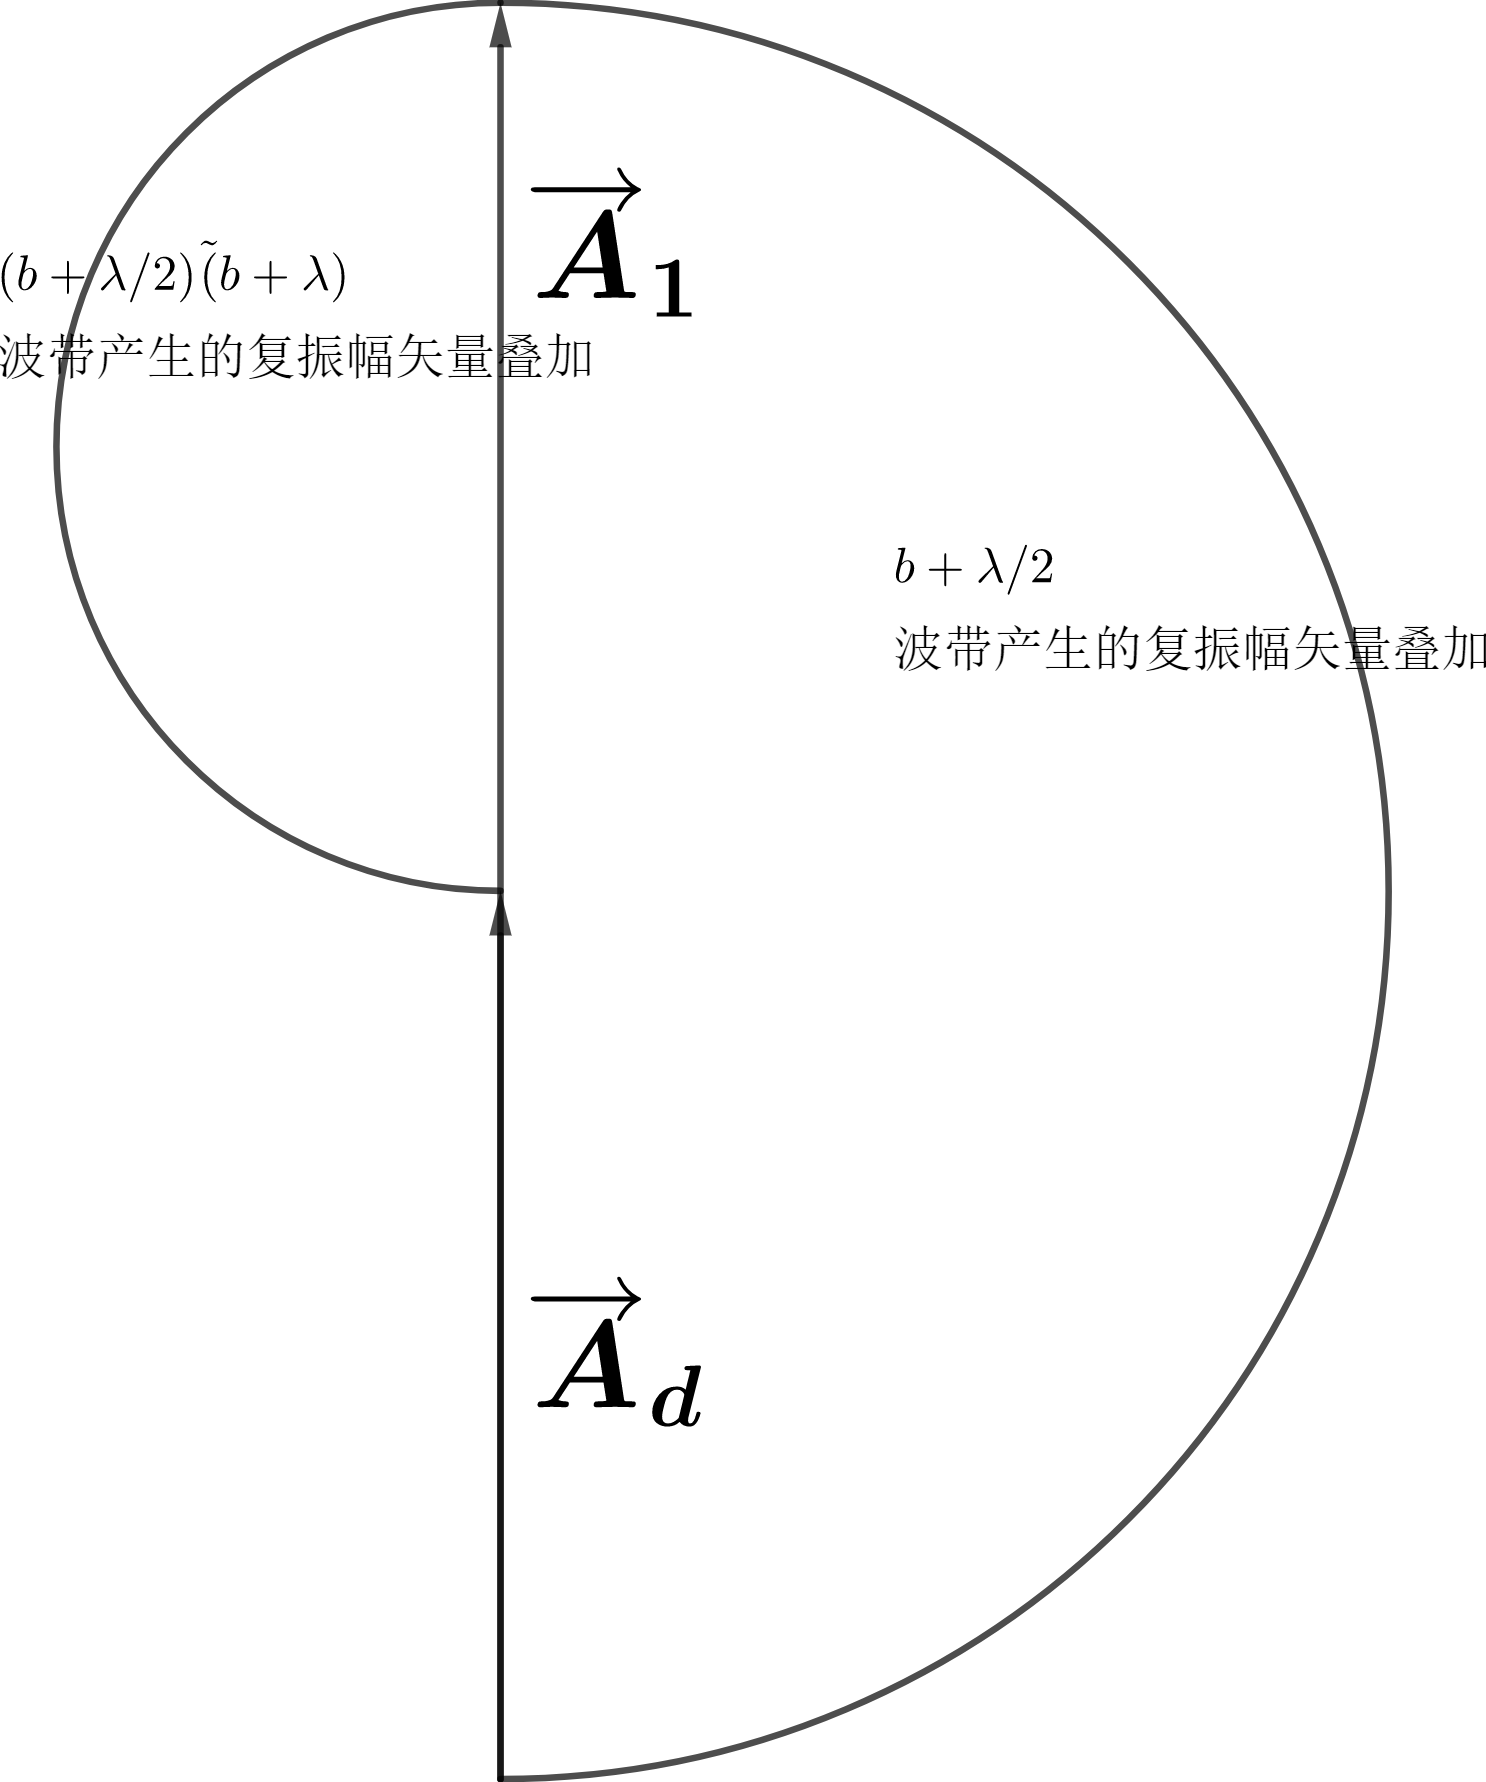
\includegraphics[scale=.12]{OpticsHomework_6_4-5d(tailored).png}
\caption{4-5d}\label{OpticsHomework_6_4-5d}
\end{figure}

\noindent 得到轴上场点的振幅为$A_d=\frac{1}{2}A_1$,光强为$I_d=A_d^2=\frac{1}{4}A_1^2$,与自由传播时之比为$\frac{I_d}{I}=1$。

\textbf{e}屏在轴上场点产生的复振幅如振动矢量图\ref{OpticsHomework_6_4-5e}所示,根据巴比涅原理,$e$屏在轴上场点产生的复振幅矢量是自由传播时产生的复振幅矢量与$(b+\lambda/2)\thicksim(b+3\lambda/4)$波带产生的复振幅矢量之差
\begin{figure}[h]
\centering
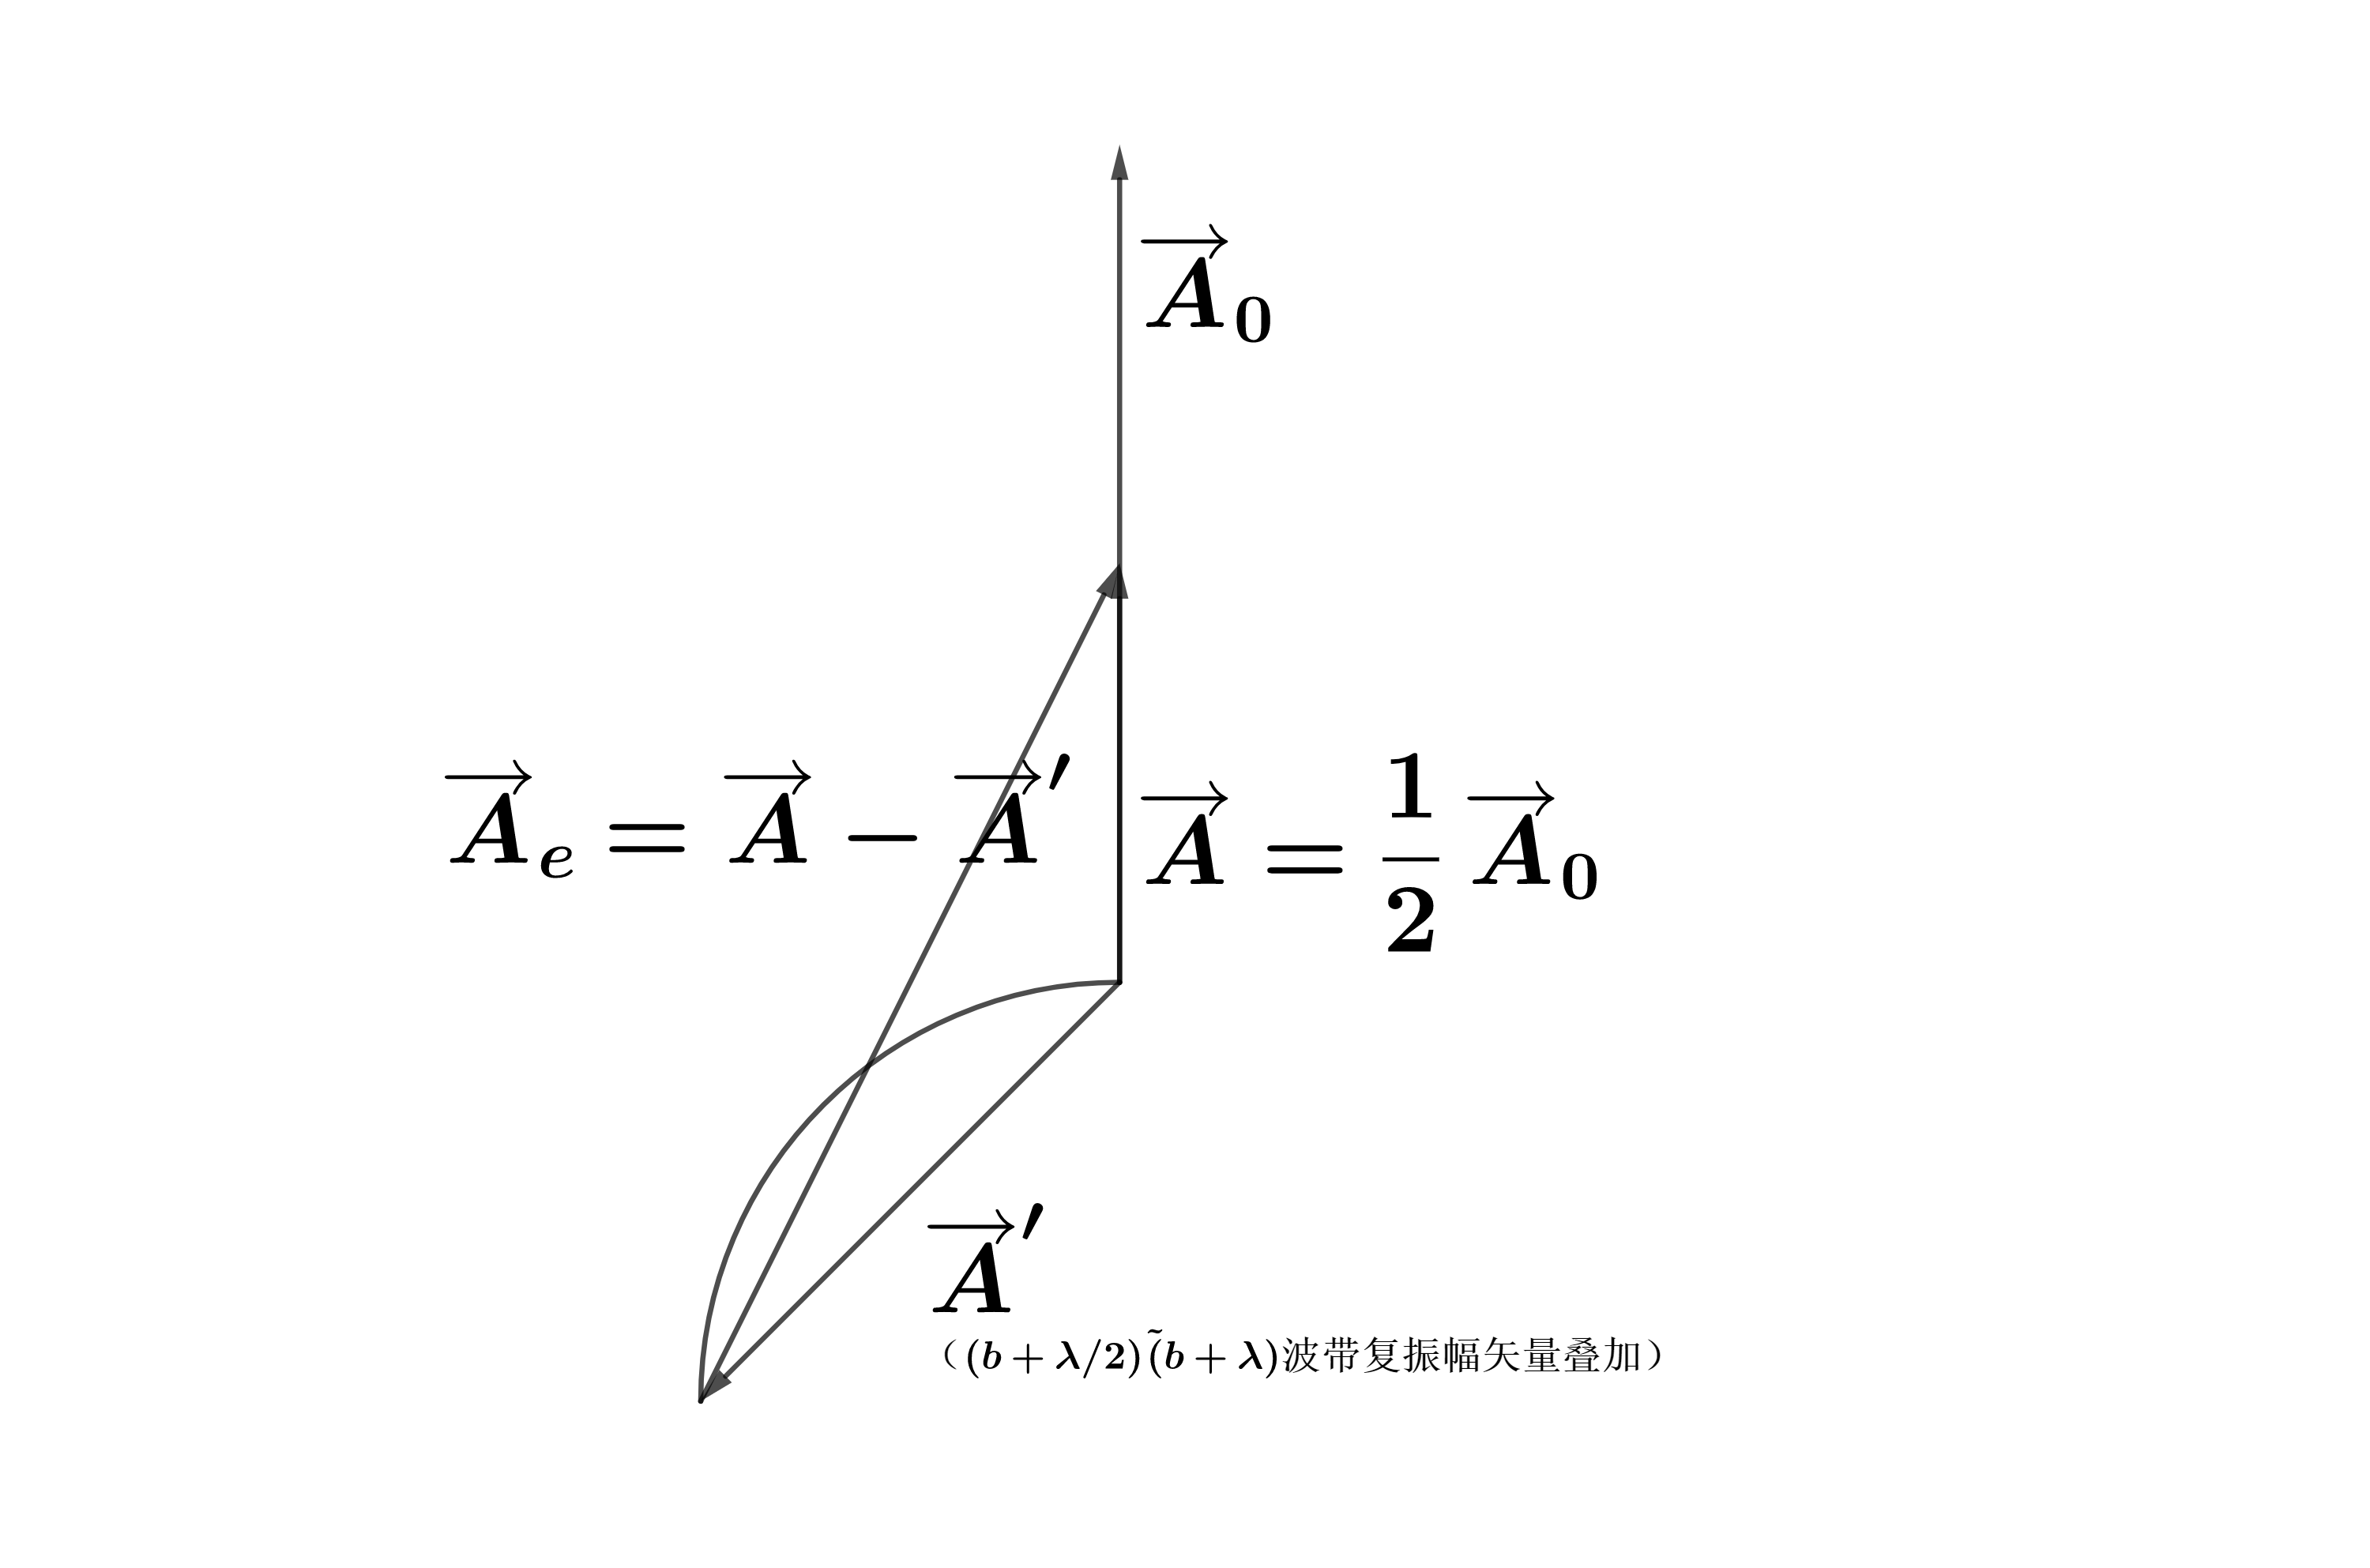
\includegraphics[scale=.15]{OpticsHomework_6_4-5e(tailored).png}
\caption{4-5e}\label{OpticsHomework_6_4-5e}
\end{figure}

\noindent 得到轴上场点的振幅为$A_e=\frac{\sqrt{5}}{2}A_1$,光强为$I_e=A_e^2=\frac{5}{4}A_1^2$,与自由传播时之比为$\frac{I_e}{I}=5$。

\textbf{f}屏在轴上场点产生的复振幅如振动矢量图\ref{OpticsHomework_6_4-5f}所示,根据巴比涅原理,$e$屏在轴上场点产生的复振幅矢量是$\frac{3}{4}$倍的自由传播时产生的复振幅矢量与$\frac{1}{4}$倍的$(b+\lambda)\thicksim(b+\lambda/2)$波带产生的复振幅矢量之和
\begin{figure}[h]
\centering
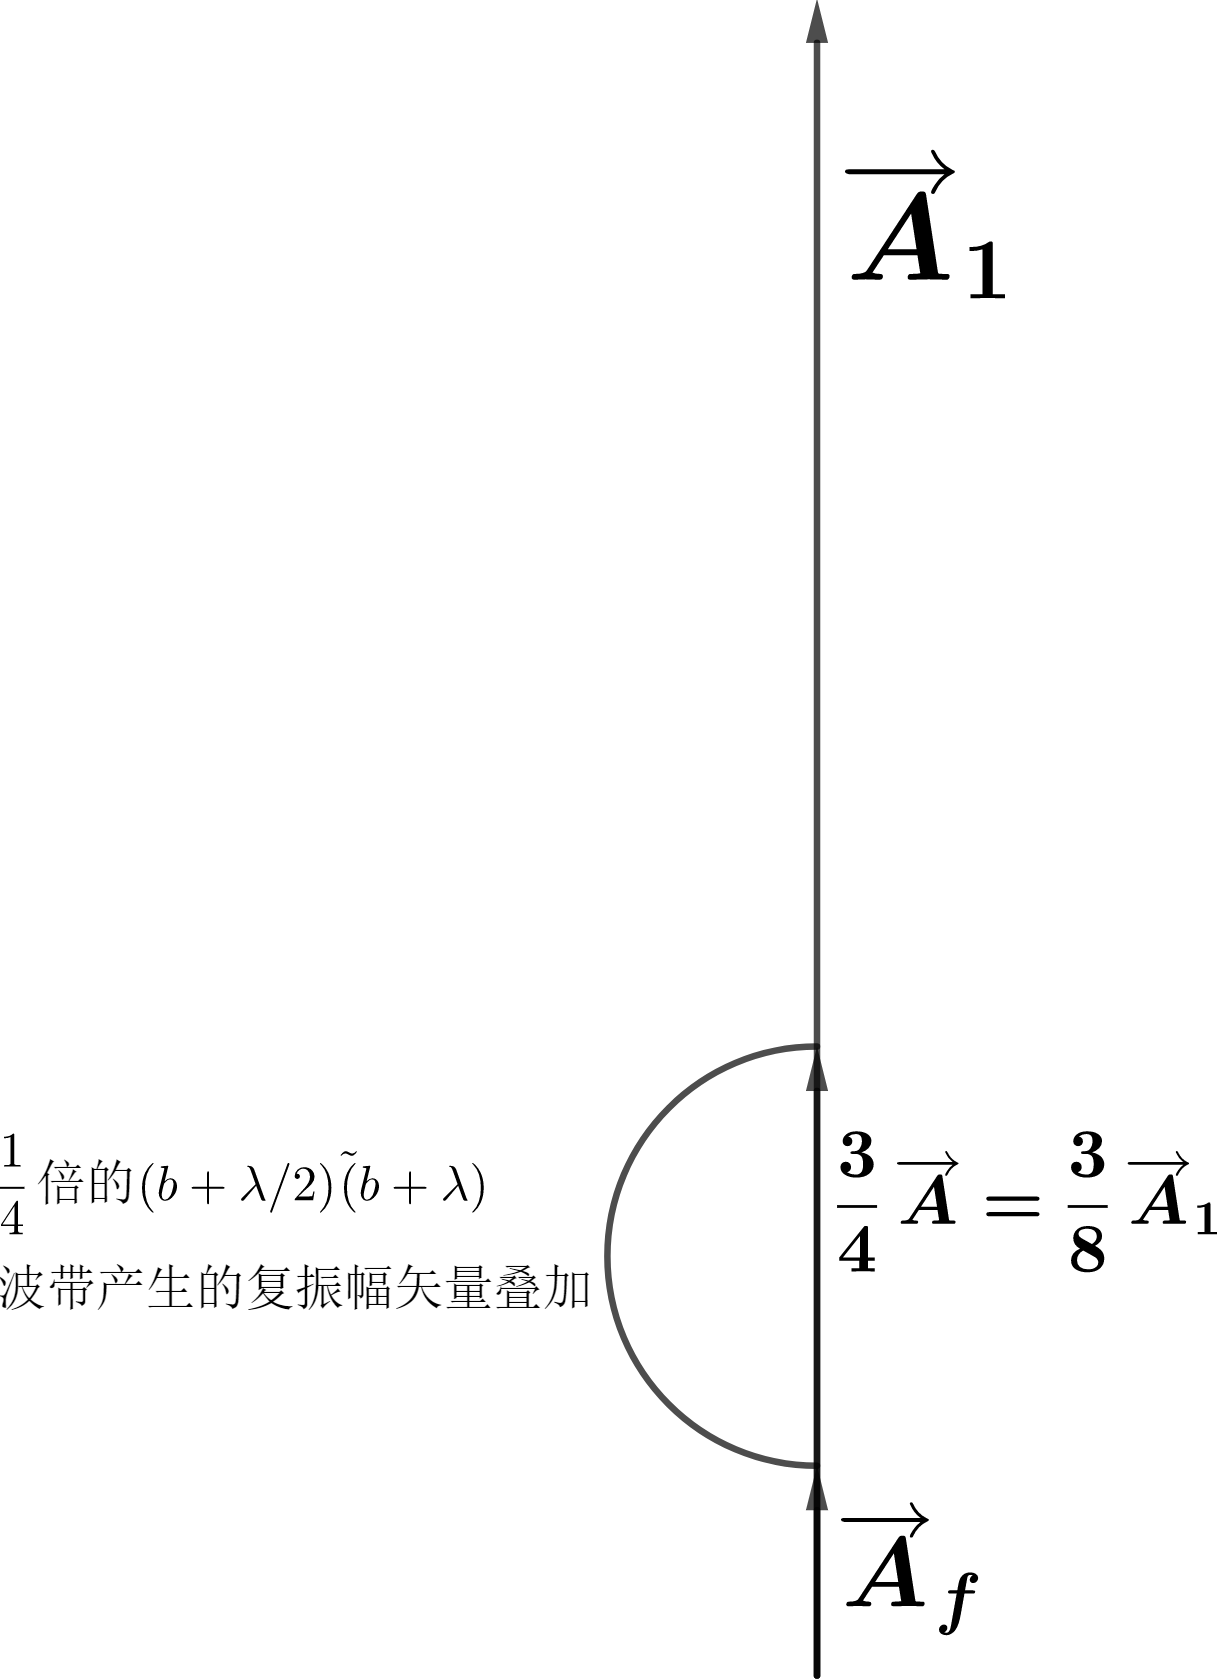
\includegraphics[scale=.15]{OpticsHomework_6_4-5f(tailored).png}
\caption{4-5f}\label{OpticsHomework_6_4-5f}
\end{figure}

\noindent 得到轴上场点的振幅为$A_f=\frac{1}{8}A_1$,光强为$I_f=A_f^2=\frac{1}{64}A_1^2$,与自由传播时之比为$\frac{I_f}{I}=\frac{1}{16}$。
\section*{4-7}解:
自由传播时衍射场中心的振幅为$A=\frac{1}{2}A_1$,强度为$I=A^2=\frac{1}{4}A_1^2$,其中$A_1$是第一个半波带在衍射场中心产生的振幅。

\noindent 根据巴比涅原理,将前$50$个奇数半波带遮挡时衍射场中心的振幅是自由传播时衍射场中心的振幅与前$50$个奇数半波带在衍射场中心产生的振幅
\[
A'=A-(A_1+A_3+...+A_{99})=-49.5A_1
\]
强度为
\[
I'=A'^2=2450.25A_1^2
\]
衍射场中心强度与自由传播时之比为
\[
\frac{I'}{I}=9801
\]
\section*{4-9}
\subsection*{(1)}解:
要求在$400nm$紫光照明下的主焦距为$80cm$,则需要第$1$级半波带的半径为
\begin{equation}
\label{equ1}
\rho_1=\sqrt{f\lambda}=0.57mm
\end{equation}
第$k$个半波带的半径为
\begin{equation}
\label{equ2}
\rho_k=\sqrt{k}\rho_1
\end{equation}
要求主焦点光强为自由传播时的$10^3$倍,则需要半波带的最高级数为
\[
n=\sqrt{10^3}\approx32
\]
对应的波带片的半径为
\[
\rho_{32}=\sqrt{32}\rho_1=3.2mm
\]
综上,以式(\ref{equ1})(\ref{equ2})的半径划分同心圆环,即为半波带,将前$32$级波带中的奇数(或偶数)波带露出,其余部分遮盖,即制成所需的半波带片。
\section*{4-10}解
第$1$级半波带的半径为
\[
\rho_1=\sqrt{f\lambda}=0.52mm
\]
改用$632.8nm$的氦氖激光照明,主焦距变为
\[
f'=\frac{\rho_1^2}{\lambda}=43cm
\]
\section*{4-11}
\subsection*{(1)}证:
如图\ref{OpticsHomework_6_4-11},经过单缝边缘两点的光路的光程差为
\[
\Delta L=a(\sin\theta-\sin\theta_0)
\]
对应的相位差为
\[
\delta=\frac{2\pi}{\lambda}\Delta L=\frac{2\pi}{\lambda}a(\sin\theta_0-\sin\theta_0)=2\alpha
\]
\begin{figure}[h]
\centering
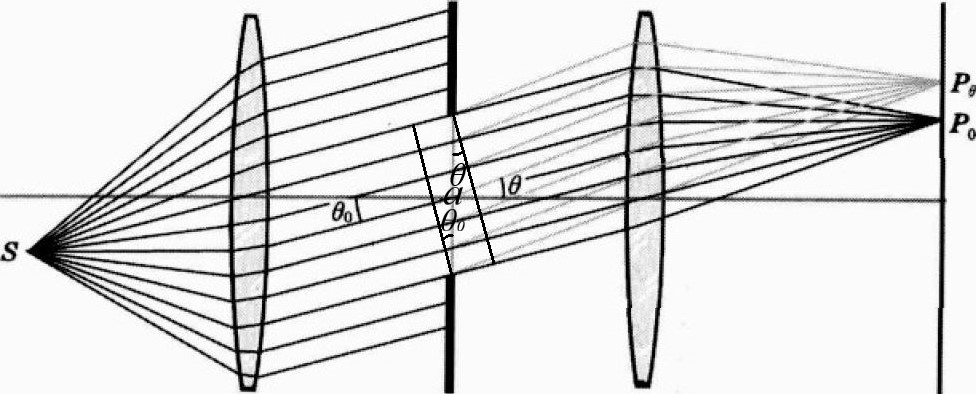
\includegraphics[scale=.4]{OpticsHomework_6_4-11.jpg}
\caption{4-11}\label{OpticsHomework_6_4-11}
\end{figure}

\noindent 根据振动矢量叠加得场点的振幅为
\[
A=2\frac{A_0}{\delta}\sin\frac{\delta}{2}=A_0\frac{\sin\alpha}{\alpha}
\]
其中$A_0$为衍射图案零级中心的振幅。场点的强度公式为
\begin{equation}
\label{equ3}
I=A^2=A_0^2(\frac{\sin\alpha}{\alpha})^2=I_0(\frac{\sin\alpha}{\alpha})^2
\end{equation}
其中$I_0$为零级中心强度,$\alpha=\frac{a\pi}{\lambda}(\sin\theta-\theta_0)$。
\subsection*{(2)}证:
根据衍射强度公式(\ref{equ3}),在$\alpha=0$处,场点强度最大,为衍射图案的零级中心;此时$\theta=\theta_0$,各条光路到像屏的光程相等,根据费马原理对应的位置即为几何光学像点处。故零级中心的位置在几何光学像点处。
\section*{(3)}证:
第$1$级暗纹对应的角宽度满足
\begin{align*}
&\alpha=\pm\pi\\
\Longrightarrow&\frac{a\pi}{\lambda}(\sin\theta_{\pm1}-\sin\theta_0)=\pm\pi\\
\Longrightarrow&\sin\theta_{\pm1}-\sin\theta_0=\pm\frac{\lambda}{a}
\end{align*}
由于$\theta_{\pm1}\to\theta$,故$\sin\theta_{\pm1}-\sin\theta_0\approx\frac{d\sin\theta}{d\theta}|_{\theta=\theta_0}(\theta_{\pm1}-\theta_0)=\cos\theta_0(\theta_{\pm1}-\theta_0)$,零级斑半角宽即为第$1$级暗纹对应的角宽度之半
\[
\Delta\theta=|\theta_{\pm1}-\theta_0|=\frac{\lambda}{a\cos\theta_0}
\]
\subsection*{(4)}证:
若单缝两侧并非同一介质,设单缝左侧介质折射率为$n_1$,右侧介质折射率为$n_2$,则经过单缝边缘两点的光路的光程差变为
\[
\Delta L'=a(n_2\sin\theta-n_1\sin\theta)
\]
对应的相位差变为
\[
\delta'=\frac{2\pi}{\lambda}\Delta L=\frac{2\pi}{\lambda}a(n_2\sin\theta-n_1\sin\theta_0)=2\alpha'
\]
故$\alpha$的定义变为$\alpha'=\frac{a\pi}{\lambda}(n_2\sin\theta-n_1\sin\theta_0)$,但强度公式仍为
\[
I=I_0(\frac{\sin\alpha}{\alpha})^2
\]
零级中心对应角度$\theta_0'$满足
\[
n_1\sin\theta_0=n_2\sin\theta_0'
\]
零级斑半角宽度变为
\begin{align*}
&n_2\sin\theta_{\pm1}-n_1\sin\theta_0=n_2(\sin\theta_{\pm1}-\sin\theta_0')=\pm\frac{\lambda}{a}\\
&\because\sin\theta_{\pm1}-\sin\theta_0'\approx\cos\theta_0'\Delta\theta\\
\Longrightarrow&\Delta\theta=\frac{\lambda}{n_2a\cos\theta_0'}=\frac{\lambda}{a\sqrt{n_2^2-n_1^2\sin\theta_0}}
\end{align*}
\section*{4-12}解:
\subsection*{(1)}解:
当平行光正入射时,反射光束的衍射发散角为
\[
\Delta\theta_1=\frac{\lambda}{a}=\frac{0.6\times10^{-6}m}{1\times10^{-2}m}=6\times10^{-5}rad\approx12.4''
\]
折射光束的衍射发散角为
\[
\Delta\theta_2=\frac{\lambda}{n_2a}=\frac{0.6\times10^{-6}m}{1.5\times1\times10^{-2}m}=4\times10^{-5}rad\approx8.2''
\]
\subsection*{(2)}解:
当入射角为$\theta_0=75^{\circ}$,反射光束的衍射发散角为
\[
\Delta\theta_1=\frac{\lambda}{a\cos\theta_0}=\frac{0.6\times10^{-6}m}{1\times10^{-2}m\times\cos75^{\circ}}=2.3\times10^{-4}rad\approx47.4''
\]
折射光束的衍射发散角为
\begin{align*}
\Delta\theta_2=\frac{\lambda}{a\sqrt{n_2^2-n_1^2\sin\theta_0}}=\frac{0.6\times10^{-6}m}{1\times10^{-2}m\times\sqrt{1.5^2-\sin^275^{\circ}}}=&5.2\times10^{-5}rad\\
\approx&10.7''
\end{align*}
\subsection*{(3)}解:
当入射角为$89^{\circ}$时,反射光束的衍射发散角为
\[
\Delta\theta_1=\frac{\lambda}{a\cos\theta_0}=\frac{0.6\times10^{-6}m}{1\times10^{-2}m\times\cos89^{\circ}}=3.4\times10^{-3}rad
\]
折射光束的衍射发散角为
\begin{align*}
\Delta\theta_2=\frac{\lambda}{a\sqrt{n_2^2-n_1^2\sin\theta_0}}=\frac{0.6\times10^{-6}m}{1\times10^{-2}m\times\sqrt{1.5^2-\sin^289^{\circ}}}=&5.4\times10^{-5}rad\\
\approx&11.1''
\end{align*}
\section*{4-17}
\subsection*{(1)}解:
取人眼最敏感的光波长$\lambda=0.55\mu m$,最小分辨距离为
\[
\delta y_{\min}=\frac{0.61\lambda}{N.A.}=0.25\mu m
\]
\subsection*{(2)}解:
人眼的明视距离为$s_0=25cm$,最小分辨角为$\delta\theta_{e}=1'$,最下分辨距离为$\delta y_{e}=s_0\delta\theta_{e}=72.7\mu m$。有效放大率为
\[
M=\frac{\delta y_e}{\delta y_{\min}}=290
\]
\subsection*{(3)}解:
当达到有效放大率时,光学筒长为
\[
\Delta=\frac{f_Of_E}{s_0}M=111mm
\]
\section*{4-19}解:
取光波长$\lambda=0.55\mu m$,该天文望远镜的最小分辨角为
\[
\delta\theta_{\min}=1.22\frac{\lambda}{D}=6.71\times10^{-7}rad
\]
能分辨月球表面两点的最小距离是
\[
\delta y_{\min}=r\delta\theta_{\min}=255m
\]
\section*{4-23}解:
由$4-11$得单缝夫琅禾费衍射的振幅公式为
\[
a_{\theta}=a_0\frac{\sin\alpha'}{\alpha'}
\]
其中$a_0$是单缝在衍射零级中心产生的振幅,$\alpha'=\frac{\pi a}{\lambda}(\sin\theta-\sin\theta_0)$。

\noindent 相邻两缝之间的光程差为
\[
\Delta L=d(\sin\theta-\theta_0)
\]
对应的相位差为
\[
\delta=\frac{2\pi}{\lambda}\Delta L=\frac{2\pi}{\lambda}d(\sin\theta-\theta_0)=2\beta'
\]
根据各缝在场点处产生的振动矢量叠加得场点的振幅
\[
A_{\theta}=2\frac{a_\theta}{2\sin\frac{\beta}{2}}\sin\frac{N\delta}{2}=a_{\theta}\frac{\sin N\sin\beta'}{\sin\beta'}=a_0\frac{\sin\alpha'}{\alpha'}\frac{\sin N\beta'}{\sin\beta'}
\]
故斜入射时夫琅禾费多缝衍射强度分布公式为
\[
I_{\theta}=A_{\theta}^2=a_0^2(\frac{\sin\alpha'}{\alpha'})^2(\frac{\sin N\beta'}{\sin\beta'})^2=I(\frac{\sin\alpha'}{\alpha'})^2(\frac{\sin N\beta'}{\sin\beta'})^2
\]
其中$\alpha'=\frac{\pi a}{\lambda}(\sin\theta-\sin\theta_0)$,$\beta'=\frac{\pi b}{\lambda}(\sin\theta-\sin\theta_0)$。
\section*{4-25}解:
单缝夫琅禾费衍射振幅公式为
\[
a_{\theta}=a_0\frac{\sin\alpha}{\alpha}
\]
$d$和$2d$的缝距对应的光程差分别为
\[
\Delta L_1=d\sin\theta, \Delta L_2=2d\sin\theta
\]
对应的相位差分别为
\[
\delta_1=\frac{2\pi}{\lambda}\Delta L_1=\frac{2\pi}{\lambda}d\sin\theta=2\beta, \delta_2=\frac{2\pi}{\lambda}\Delta L_2=\frac{2\pi}{\lambda}2d\sin\theta=4\beta
\]
如图\ref{OpticsHomework_6_4-25},根据振动矢量叠加,解得总振动矢量的$x,y$分量分别为
\begin{align*}
&A_{\theta x}=a_{\theta}(1+\cos\delta_1+\cos(\delta_1+\delta_2))=a_{\theta}(1+\cos2\beta+\cos6\beta)\\
&A_{\theta y}=a_{\theta}(\sin\delta_1+\sin(\delta_1+\delta_2))=a_{\theta}(\sin2\beta+\sin6\beta)
\end{align*}
\begin{figure}[h]
\centering
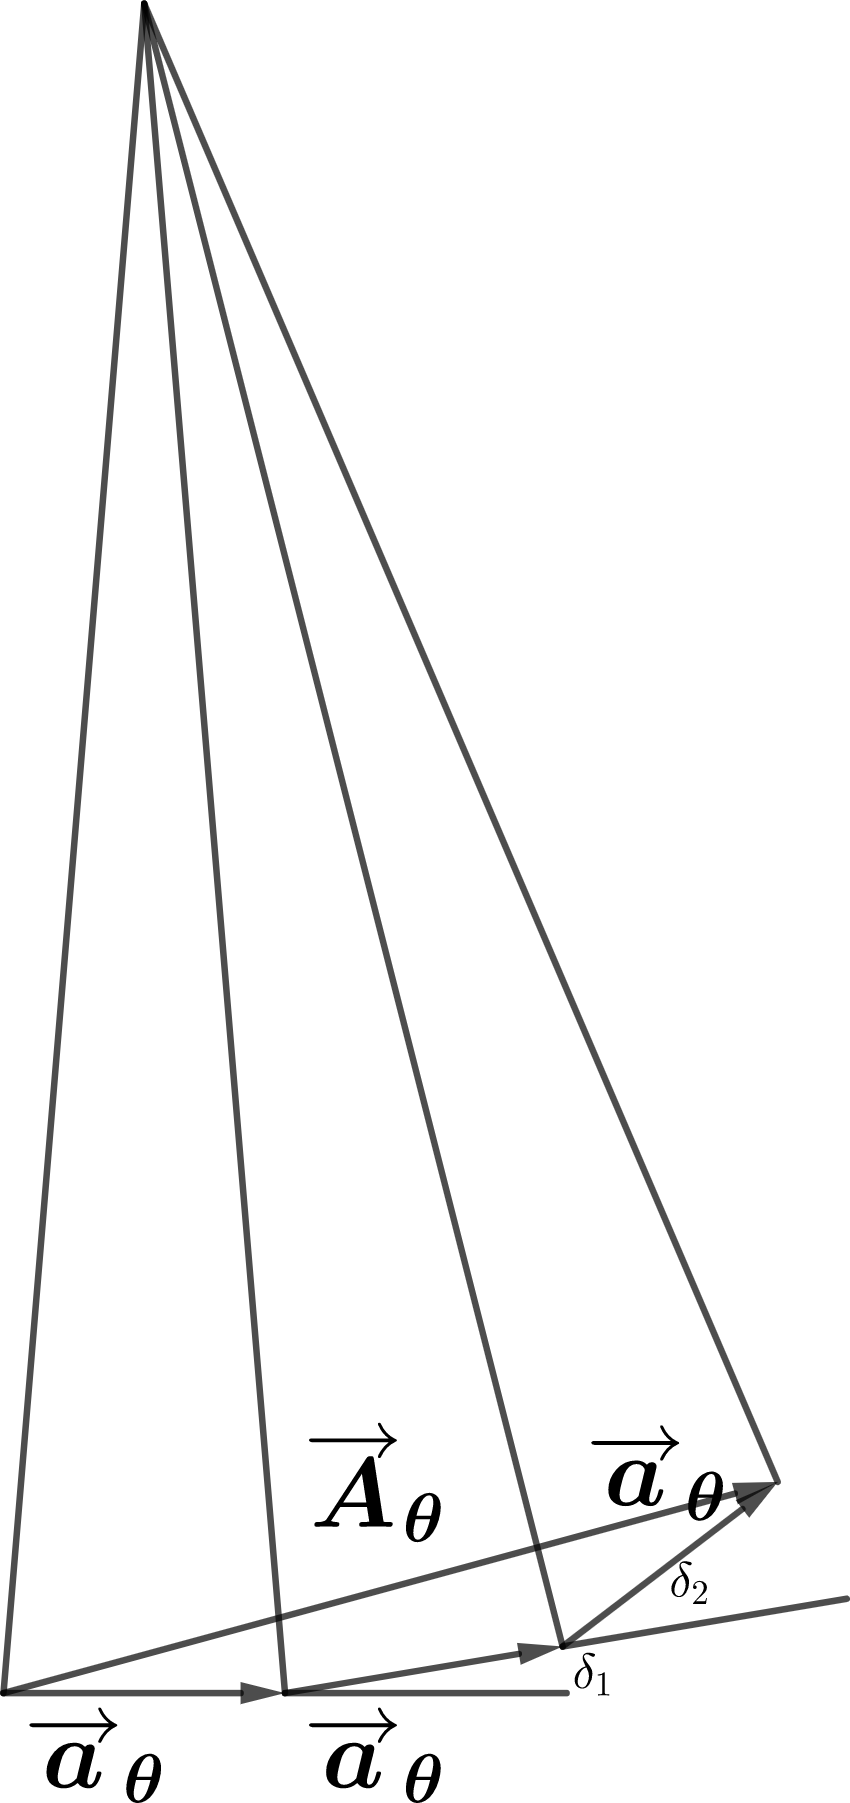
\includegraphics[scale=.1]{OpticsHomework_6_4-25(tailored).png}
\caption{4-25}\label{OpticsHomework_6_4-25}
\end{figure}

\noindent 总振幅为
\begin{align*}
A_{\theta}=&\sqrt{A_{\theta x}^2+A_{\theta y}^2}=a_{\theta}^2[(1+\cos2\beta+\cos6\beta)^2+(1+\sin2\beta+\sin6\beta)^2]\\
=&a_0^2(\frac{\sin\alpha}{\alpha})^2[3+2(\cos2\beta+\cos4\beta+\cos6\beta)]\\
=&I_0(\frac{\sin\alpha}{\alpha})^2[3+2(\cos2\beta+\cos4\beta+\cos6\beta)]
\end{align*}
\section*{4-27}
\subsection*{(1)}解:
遮住偶数缝时,相当于缝宽为$a$,缝间距为$6a$的多缝夫琅禾费衍射,其强度分布公式为
\[
I_{\theta}=I_0(\frac{\sin\alpha}{\alpha})^2(\frac{\sin N\beta}{\sin\beta})^2
\]
其中$\alpha=\frac{\pi a}{\lambda}\sin\theta$,$\beta=\frac{6\pi a}{\lambda}\sin\theta$。
\subsection*{(2)}解:
遮住奇数缝时,同样相当于相当于缝宽为$a$,缝间距为$6a$的多缝夫琅禾费衍射,其强度分布公式同上
\[
I_{\theta}=I_0(\frac{\sin\alpha}{\alpha})^2(\frac{\sin N\beta}{\sin\beta})^2
\]
其中$\alpha=\frac{\pi a}{\lambda}\sin\theta$,$\beta=\frac{6\pi a}{\lambda}\sin\theta$。
\subsection*{(3)}解:
当全开放时,相当于前两题的叠加,根据振动矢量叠加得强度分布公式为
\[
I_{\theta}'=I_{\theta}(2\sin(\frac{\pi}{2}-2\alpha))^2=4I_0\cos^22\alpha(\frac{\sin\alpha}{\alpha})^2(\frac{\sin N\beta}{\sin\beta})^2
\]
\section*{4-32}
\subsection*{(1)}解:
该摄谱仪在第一级光谱在闪耀波长附近能分辨的谱线间隔的最小值为
\[
\delta\lambda=\frac{\lambda}{R}=5.1\times10^{-3}nm
\]
\subsection*{(2)}解:
该摄谱仪的线色散本领为$D_l=\frac{1}{0.8nm/mm}=1.25mm/nm$,角色散本领为
\[
D_{\theta}=\frac{D_l}{f}=4.1'/mm
\]
\subsection*{(3)}解:
光栅常数为
\[
d=\frac{1}{1200mm^{-1}}=8.3\times10^{2}mm
\]
光栅的闪耀角为
\[
\theta_b=\arcsin\frac{\lambda_1b}{2d}=12^{\circ}39'
\]
闪耀方向与光栅平面的法线方向所成角度与之相同,为$12^{\circ}39'$。
\section*{3-34}
\subsection*{(1)}解:
光栅的色分辨本领为
\[
R_{\text{光栅}}=kN=1\times5\times10^{-2}m\times600\times1000m^{-1}=3\times10^4
\]
棱镜的色分辨本领为
\[
R_{\text{棱镜}}=b\frac{dn}{d\lambda}=5\times10^{-2}m\times0.6\times10^{-4}\times10^9m^{-1}=3\times10^3
\]
取光波长$\lambda=0.55\mu m$,正入射,对于第$1$级干涉条纹,法-珀干涉仪的色分辨本领为
\[
R_{F-P}=\frac{\lambda}{\delta\lambda}=\frac{2\pi nh}{\lambda}\frac{\sqrt{R}}{1-R}=\frac{2\pi\times1\times5\times10^{-2}m}{5.5\times10^{-7}m}\frac{\sqrt{0.99}}{1-0.99}=6\times10^7
\]
色分辨本领比较:
\[
R_{F-P}>R_{\text{光栅}}>R_{\text{棱镜}}
\]
\subsection*{(2)}解:
光栅的角色散本领为
\[
D_{\text{光栅}}=\frac{k}{d\cos\theta_k}=\frac{1}{1/(600mm^{-1})}=2.2'/nm
\]
棱镜的角色散本领为
\begin{align*}
D_{\text{棱镜}}=\frac{2\sin(\alpha/2)}{\sqrt{1-n^2\sin^2(\alpha/2)}}\frac{dn}{d\lambda}=&\frac{2\sin30^{\circ}}{\sqrt{1-1.5^2\sin^230^{\circ}}}\times0.6\times10^{-4}\times10^9m^{-1}\\
=&0.31'/nm
\end{align*}
对于第$1$级干涉条纹,取$i_k=10^{\circ}$,法-珀干涉仪的角色散本领为
\[
D_{F-P}=\frac{di_k}{d\lambda}=\frac{k}{2nh\sin i_k}=\frac{2nh\cos i_k}{2nh\lambda\sin i_k}=\frac{\cot10^{\circ}}{5.5\times10^{-7}m}=35.5'/nm
\]
角色散本领比较:
\[
D_{F-P}>D_{\text{光栅}}>D_{\text{棱镜}}
\]
\subsection*{(3)}解:
光栅的自由光谱范围为
\[
\lambda\in[\frac{d}{2},d]=[\frac{1/(600mm^{-1})}{2},1/(600mm^{-1})]=[850.0nm,1700.0nm]
\]
棱镜只有一套光谱,故不存在不同级光谱之间的重叠,从而自由光谱范围不受限制。

\noindent 法珀干涉仪的自由光谱范围为
\begin{align*}
&k\lambda=(k-1)(\lambda+\delta\lambda)\\
\Longrightarrow&\delta\lambda=\frac{\lambda}{k-1}\approx\frac{\lambda^2}{2nh}=\frac{(5.5\times10^{-7}m)^2}{2\times1\times5\times10^{-2}m}=0.003nm
\end{align*}
故棱镜的自由光谱范围大于光栅的自由光谱范围大于法-珀干涉仪的自由光谱范围。
\end{document}
